\documentclass[a4paper, 11pt]{article}
\usepackage[utf8]{inputenc}
\usepackage[slovak]{babel}
\usepackage{graphicx}
\usepackage{xcolor}
\usepackage[unicode]{hyperref}
\usepackage[left=2cm, top=3cm, text={17cm, 24cm}]{geometry}
\hypersetup{
	colorlinks = true,
	linkcolor = blue,
	citecolor = red,
        urlcolor = blue
}
%%%%%%%%%% Numbering %%%%%%%%%%%%%%%%%%%%%%%
\usepackage{titlesec}
\setcounter{secnumdepth}{4}

\titleformat{\paragraph}
{\normalfont\normalsize\bfseries}{\theparagraph}{1em}{}
\titlespacing*{\paragraph}
{0pt}{3.25ex plus 1ex minus .2ex}{1.5ex plus .2ex}
%%%%%%%%%%%%%%%%%%%%%%%%%%%%%%%%%%%%%%%%%%%%%

\title{ISA - Projektová dokumentácia}
\author{xhoril01}
\date{October 2022}

\begin{document}

    %%%%%%%% Titulná stránka %%%%%%%%%%%
    \begin{titlepage}
        \begin{center}
            
\includegraphics[width=0.8\linewidth]{./img/VUT_LOGO} \\
            
			\vspace{\stretch{0.5}}

			\Huge{Projekt ISA 2022} \\
			\LARGE{\textbf{Čítačka noviniek vo formáte Atom a~RSS s~podporou TLS}} \\

			\vspace{\stretch{0.8}}
		\end{center}

		{\Large
			\today
			\hfill
			Denis Horil (xhoril01)
		}
    \end{titlepage}

    %%%%%%%%%%%%%%%%%%%%%%%%%%%%%%%%%%%%%%%
    %%%%%%%%%%%%%%%% Obsah %%%%%%%%%%%%%%%%
    \pagenumbering{roman}
    \color{black}
    \setcounter{page}{1}
    \tableofcontents
    \clearpage

    %%%%%%%%%%%%%%%%%%%%%%%%%%%%%%%%%%%%%%%
    %%%%%%%%%%%%%%%% Úvod %%%%%%%%%%%%%%%%%
    \pagenumbering{arabic}
    \setcounter{page}{1}
    \section{Úvod}
    \label{intro}

    Cieľom projektu bolo vytvoriť program \texttt{feedreader} v C/C++, ktorý bude vypisovať požadované informácie z tzv. \texttt{feedov}. Informácie sú uvedené v XML súboroch vo formáte RSS 2.0 \cite{rss2} alebo Atom \cite{atom}. \\

    %%%%%%%%%%%%%%%%%%%%%%%%%%%%%%%%%%%%%%%
    %%%%%%%%%%%%%%% Popis %%%%%%%%%%%%%%%%%
    \section{Popis vstupného súboru}
    \label{feeds}

    Ako bolo spomenuté v \ref{intro}, program stiahne informácie z webovej adresy (angl. \texttt{feed}) a vypíše ich.\\

    Internetový \textit{feed} je formát dokumentu, ktorý dovoľuje publikáciu zoznamov s informáciami alebo konkrétnymi prepojeniami \footnote{https://www.mnot.net/rss/tutorial/}. Tento dokument obsahuje informácie o \textit{feede} samotnom (tzv. \textit{metadata}) - nadpis daného \textit{feedu}, jeho autora, dátum publikácie a kde ho vieme~nájsť na internete. Za tým nasleduje zoznam \textbf{prvkov}(tzv. \textit{item}) a \textbf{vstupov}(tzv. \textit{entry}).\\
    
    Bežný prvok obsahuje \textit{link}, \textit{nadpis} a \textit{popis}. Množstvo prvkov obsahuje aj iné \textit{metadata} napr. dátum publikácie alebo meno či email autora. \\
    
    Najčastejšie používané formáty feedov sú \textbf{RSS2.0} alebo \textbf{Atom}.

    \subsection{RSS}
    \label{RSS}
    
    \textbf{RSS} je publikovací formát obsahu na internete. Skratka \textit{RSS} je akronymom pre "Really Simple Syndication" (\textit{Naozaj jednoduchá publikácia}). Tento formát je "dialektom" XML formátu a preto musí odpovedať špecifikácii XML 1.0\footnote{https://www.w3.org/TR/REC-xml/}.
    Formát \textit{RSS} má niekoľko verzií \footnote{https://www.rssboard.org/rss-history}:
    \begin{itemize}
        \item RSS 0.90
        \item RSS 0.91
        \item RSS 0.92
        \item RSS 1.0
        \item RSS 2.0
    \end{itemize}
    
    Napriek spoločnému názvu RSS sa jednotlivé verzie líšia, a to najmä v prvkoch (\textit{elementoch}). \\
    
    \subsubsection{RSS 1.0}
    Verzia 1.0 bola založená na verzii 0.90 a aby si ju osvojili tvorcovia obsahu, bola zabezpečená aj spätná kompatibilita týchto 2 verzií \footnote{https://validator.w3.org/feed/docs/rss1.html\#s7}. \\
    
    Verzia RSS 1.0 obsahuje koreňový prvok \texttt{<rdf:RDF>}, v ktorom je povinný prvok \texttt{<title>}. Spoločný s ostatnými verziami je však prvok \texttt{<channel>}, ktorý sa vyskytuje aj v tejto verzii len raz. Narozdiel od verzie RSS 2.0 sa prvky \texttt{<item>} nachádzajú na rovnakej úrovni ako prvok \texttt{<channel>}.
    Prvok \texttt{<item>} musí obsahovať 2 prvky:
    \begin{itemize}
        \item \texttt{<title>}
        \item \texttt{<link>}
        \item \texttt{<description>}
    \end{itemize}
    
    \subsubsection{RSS 2.0}
    Verzia 2.0 bola založená na verzii 0.91, takže aj tu je zabezpečená spätná kompatibilita, no medzi verziami 1.0 a 2.0 spätná kompatibilita \textbf{NIE JE} zabezpečená\cite{rss2}.\\
    
    Verzia RSS 2.0 (a teda aj RSS 0.91 a 0.92) obsahuje koreňový prvok \texttt{<rss>}, kde je povinne uvedená daná verzia. V tomto koreňovom prvku sa nachádza jediný prvok \texttt{<channel>}, v ktorom je povinný prvok \texttt{<title>}.
    Všetky prvky \texttt{<item>} sú podprvkami prvku \texttt{<channel>}. Povinné prvky \texttt{<item>} sú:
    \begin{itemize}
        \item \texttt{<title>}
        \item \texttt{<link>}
        \item \texttt{<description>}
    \end{itemize}
    Vo verzii RSS 0.91 nie sú informácie o autorovi alebo dátum úpravy podporované, vo verzii RSS 0.92 boli pridané niektoré nepovinné prvky a vo verzii RSS 2.0 sú podporované nepovinné prvky:
    \begin{itemize}
        \item \texttt{<author>}
        \item \texttt{<pubDate>}
    \end{itemize} 

    \subsection{Atom}
    \label{Atom}
    
    \textbf{Atom} je publikovací formát založený na báze XML, ktorý popisuje zoznamy súvisiacich informácii - \texttt{feedov}. \texttt{Feedy} pozostávajú z viacerých prvkov tzv. \textit{vstupov} (angl. \texttt{entry}). Každý takýto prvok obsahuje rozšíriteľnú množinu pripojených metadát napr. každý \texttt{entry} má nadpis (\texttt{title})\footnote{https://datatracker.ietf.org/doc/html/rfc4287}. \\

    Koreňovým elementom je prvok \texttt{<feed>}. Ten musí obsahovať 3 povinné prvky:
    \begin{itemize}
        \item \texttt{<id>} - identifikuje \textit{feed} unikátnou a permanentnou URI \cite{URI}
        \item \texttt{<title>} - titulok/názov \textit{feedu}
        \item \texttt{<updated>} - posledná úprava \textit{feedu}
    \end{itemize}
    Po predchadzájúcich metadátach nasleduje ľubovoľný počet prvkov \texttt{<entry>}, ktoré reprezentujú jednotlivé položky zdroja. \\ 
    
    Každý prvok \texttt{<entry>}, rovnako ako \texttt{<feed>}, musí obsahovať 3 povinné prvky \texttt{<id>}, \texttt{<title>} a \texttt{<updated>}.
    Ďalej sú odporúčané aj prvky: 
    \begin{itemize}
        \item \texttt{<author>} - uvádza jedného autora \textit{feedu}
        \item \texttt{<content>} - obsahuje kompletný obsah prvku \texttt{<entry>}
        \item \texttt{<link>} - identifikuje asociovanú URL
        \item \texttt{<summary>} - poskytuje krátke zhrnutie, abstrakt alebo úryvok zo záznamu
    \end{itemize}
    Pri prvku \texttt{<author>} je to ale trochu zložitejšie. Každý prvok \texttt{<entry>} môže obsahovať viacerých autorov alebo aj žiadneho. Prvok \texttt{<author>} obsahuje povinne prvok \texttt{<name>} (meno autora) a nepovinne \texttt{<email>} (email autora) alebo \texttt{<uri>}(domovská stránka autora). Pokiaľ nie je uvedený autor, použije sa autor z prvku \texttt{<source>}. Ak ani ten nie je uvedený, použije sa autor uvedený v prvku \texttt{<feed>}.
    
    %%%%%%%%%%%%%%%%%%%%%%%%%%%%%%%%%%%%%%%
    %%%%%%%%%%%% Implementácia %%%%%%%%%%%%
    \section{Implementácia}
    \label{implementation}

    Program \texttt{feedreader} je čítačkou noviniek vo formáte Atom \ref{Atom} a RSS \ref{RSS} s podporou TLS. Program po spustení stiahne zadané zdroje a vypíše na štandardný výstup informácie požadované úživateľom (napr. názvy článkov). \\
    
    Program je implementovaný v C++, a teda je využitý objektovo orientovaný prístup. Celý program je implementovaný v 2 súboroch: \texttt{feedreader.cpp} a \texttt{classes.cpp}.

    \subsection{\texttt{feedreader.cpp}}
    \label{feedreader}
    Súbor \texttt{feedreader.cpp} je hlavným súborom, ktorý spúšťa celú čítačku. V tomto súbore sú definované 2 funkcie: \texttt{prog\_interrupt} a \texttt{main}. \\
    Funkcia \texttt{prog\_interrupt} zabezpečuje uvoľnenie pamäte pri nečakanom ukončení programu (CTRL+C). \\
    
    Funkcia \texttt{main} vytvorí inštancie tried \textit{Args} \ref{Args} a \textit{Process} \ref{Process}. Táto funkcia vyvolá postupne funkcie na spracovanie vstupných argumentov a stiahnutie \textit{feedov} zo zadaných zdrojov.\\

    \subsection{\texttt{classes.cpp}}
    \label{classes}
	V súbore \texttt{feedreader.cpp} sú implementované triedy a všetky pomocné funkcie a štruktúry. Takisto sú tu definované makrá pre výpis chybových stavov a uvoľnenie pamäte po vyvolaní chyby.
	
    \subsubsection{Makrá}
    \label{macros}
    V celom programe sú použité 3 makrá - \texttt{ERR\_STAT}, \texttt{ERR\_STAT\_ARG} a \texttt{IM\_FREEEEE}. \\
    \texttt{ERR\_STAT} je makro pre výpis chybovej hlášky na štandardný chybový výstup bez parametra. \\
    \texttt{ERR\_STAT\_ARG} je podobne ako \texttt{ERR\_STAT} makro pre výpis chybovej hlášky na štandardný chybový výstup, ale s pridaným parametrom, ktorý sa má vypísať. \\
    \texttt{IM\_FREEEEE} je makro, ktoré uvoľní pamäť alokovanú pri vytváraní pripojenia na zadanú webovú adresu. \\
	
    \subsubsection{Pomocné funkcie}
    \label{functions}
    Ďalej sú definované funkcie \texttt{schemeCheck} a \texttt{checkURL}, ktoré slúžia na kontrolu správnosti zadanej URL.\\
    Funkcia \texttt{schemeCheck} skontroluje, či je správny protokol pre sťahovanie zdrojov. Povolené protokoly sú \textit{HTTP} a \textit{HTTPS}..\\
    Funkcia \texttt{checkURL} skontroluje správnosť zadanej URL, rozloží URL na jednotlivé zložky a uloží tieto zložky do štruktúry  \texttt{parsedURL} \ref{parsedURL}. Pokiaľ vrámci URL nebolo špecifikované číslo portu, implicitne sa použije číslo portu pre daný protokol tj. 80 pre protokol \textit{HTTP} a 443 pre \textit{HTTPS}

    \subsubsection{Pomocné štruktúry}
    \label{structures}
    Štruktúry uvedené nižšie slúžia zväčša na uloženie infromácií pre lepšiu manipuláciu s danými dátami.	

    \paragraph{\texttt{parsedURL}}
    \label{parsedURL}
    V tejto štruktúre je uložená URL rozložená na jednotlivé časti. URL sa skladá z:
    \begin{itemize}
	\item Protokol (\textit{scheme}) - protokol \textit{HTTP} alebo \textit{HTTPS}
	\item Doména (\textit{host}) - napr. \texttt{www.vutbr.cy}
	\item Číslo portu (\textit{port}) - ak nie je zaané, implicitne sa nastaví podľa protokolu		
	\item Cesta (\textit{path}) - cesta k danému \textit{feedu} napr. s príponou \texttt{.atom}
	\item Autorita (\textit{authority}) - kombinácia v tvare \texttt{host:port}
    \end{itemize}	

    \paragraph{\texttt{Feed}}
    \label{structFeed}
    Táto štruktúra slúži na uloženie cesty k užívateľom zadanému \texttt{feedfile} a na uloženie zoznamu validných URL zdrojov, ktoré boli zadané v \texttt{feedfile}.

    \paragraph{\texttt{Author}}
    \label{author}
    Štruktúra \texttt{Author} uchováva v sebe informácie o autorovi aktuálneho \textit{feedu} - jeho meno resp. jeho email.

    \paragraph{\texttt{XMLContent}}
    \label{content}
    V štruktúre \texttt{XMLContent} sú uložené všetky informácie o danom \textit{feede}. Slúži na výpis užívateľom požadované informácie. Štruktúra si uchováva názov aktuálneho \textit{feedu}, zoznam jeho autorov, zoznam asociovaných URL a taktiež dátum poslednej úpravy.

    \subsubsection{Trieda \textit{Args}}
    \label{Args}
    V triede \textit{Args} sú implementované všetky funkcie potrebné pre spracovanie argumentov zadané užívateľom na príkazovom riadku. \\ 

    Hlavnou funkciou je funkcia \texttt{argsProcesser()}, ktorá pomocou funkcie \texttt{getopt\_long()}\footnote{https://www.gnu.org/software/libc/manual/html\_node/Getopt-Long-Option-Example.html} identifikuje vstupné argumenty zadané na príkazovom riadku \ref{start}. Podľa zadaných argumentov sa uložia jedntolivé parametry do premenných. 
	
    Po úspešnom uložení parametrov a argumentov sa skontroluje funkciou \texttt{reqArgsCheck()} či bol zadaný aspoň jeden z povinných parametrov. \\
	
    Ďalej je tu implementovaná funkcia \texttt{printHelp()}, ktorá vypíše nápovedu na štandardný výstup a takisto funkcie štýlu "\textit{getters}" - tieto funkcie vrátia zadaný argument či parameter (napr. funckia \texttt{getURL()} vráti zadanú URL adresu alebo funkcia \texttt{isTime()} vráti, či bol alebo nebol zadaný parameter \textit{-T}). \\

    \subsubsection{Trieda \textit{Process}}
    \label{Process}
    V triede \textit{Process} sú implementované všetky funkcie potrebné pre získanie zadaných informácií. V závislosti na zadaných parametroch sú 2 spúšťacie "metódy": 
    \begin{itemize}
        \item 1. - bola zadaná URL a teda rovno je možné spustiť hlavnú funkciu \texttt{connect()} \ref{connect}
	\item 2. - bol zadaný argument \textit{-f <feedfile>} a treba najskôr získať URL z \textit{feedfile}
    \end{itemize}
	
    V prípade 2. metódy bude spustená funkcia \texttt{feedfile2List()}. Táto funkcia zo zadaného súboru \textit{feedfile} vytiahne všetky URL adresy a uloží do zoznamu v štruktúre \texttt{Feed} \ref{structFeed}. Ďalej bude vyvolaná funkcia \texttt{loopConnect()}, ktorá iteruje cez uloženy zoznam URL adries, kontroluje ich a posiela do funkcie \texttt{connect()} \ref{connect}. \\

    \paragraph{Funkcia \texttt{connect()}}
    \label{connect}
    Funkcia \texttt{connect()} zabezpečuje pripojenie (či už zabezpečené alebo nie) na zadanú URL adresu a sťahuje z nej \textit{feedy}. Pripojenie sa uskutočňuje pomocou knižnice \texttt{OpenSSL}, ktorá využíva pripojenie cez \textit{BIO} sokety\cite{openSSL}. \\

    Po úspešnom pripojení na server sa do premennej \texttt{response} načíta celá odpoveď zo serveru a spracuje sa vo funkcii \texttt{responseProcess()} \ref{responseProc}. Po úspešnom spracovaní odpovede nastáva "parsovanie" obsahu vráteného funkciou \texttt{responseProcess()} vo funkcii \texttt{parseXML()} \ref{parse}. V tejto funkcii sa priamo volá aj funkcia pre výpis požadovaných informácii. \\

    \paragraph{Funkcia \texttt{responseProcess()}}
    \label{responseProc}
    Funkcia \texttt{responseProcess()} oddelí hlavičku a obsah\textit{HTTP} odpovede a obsah v tvare popísanom v sekcii \ref{feeds} vráti do funkcie \texttt{connect()}. 

    \paragraph{Funkcia \texttt{parseXML()}}
    \label{parse}
    Táto funkcia zodpovedá za parsovanie \textit{feedu} v tvare XML s pomocou knižnice \texttt{libxml2}. S pomocou funkcie \texttt{xmlParseDoc()} sa sparsuje zadaný \textit{feed} a pomocou funkcie \texttt{xmlDocGetRootElement()} sa získa koreňový prvok. \\
    
    Na základe koreňového prvku sa rozhodne, akým štýlom sa daný \textit{feed} bude parsovať - Atom alebo RSS2.0 . (v kóde je implementovaná aj funkcia na parsovanie RDF/RSS1.0 \textit{feedu}, ale je zakomentovaná z dôvodu že tento typ nie je presne určený v zadaní projektu).\\

    Po úspešnom parsovaní funkcia \texttt{printInfo()} vypíše požadované informácie na štandardný výstup podľa formátu určeného v zadaní \ref{output}. 

    %%%%%%%%%%%%%%%%%%%%%%%%%%%%%%%%%%%%%%%
    %%%%%%%%%%%%%% Spustenie %%%%%%%%%%%%%%
    \section{Spustenie programu}
    \label{start}
    Program sa spúšťa cez príkazový riadok na platforme Linux. Možnosti spustenia preloženeého programu: \\
    \texttt{feedreader <URL | -f <feedfile>> [-c <certfile>] [-C <certaddr>] [-T] [-a] [-u]} \\
    kde: \\
    \begin{itemize}
        \item \texttt{URL} - URL adresa daného \textit{feedu}
        \item \texttt{-f <feedfile>} - cesta k súboru s URL adresami zdrojov \ref{feedfile}
        \item \texttt{-c <certfile>} - cesta k súboru s certifikátmi
        \item \texttt{-C <certaddr>} - cesta k adresáru s certifikátmi
        \item \texttt{-T} - vypíšu sa aj informácie o čase poslednej zmeny daného záznamu
        \item \texttt{-a} - vypíše sa autor daného záznamu (ak bol zadaný) alebo jeho email (ak bol zadaný)
        \item \texttt{-u} - vypíšu sa asociované URL s daným záznamom
    \end{itemize}
    Pri spustení na poradí parmetrov záleží, no musí byť uvedený jeden z parametrov \texttt{URL} alebo \texttt{-f <feedfile>}, nie však oba. Ak nebude zadaný ani jeden z parametrov \texttt{-c <certfile>} alebo \texttt{-C <certaddr>}, na získanie certifikátov bude použitá funkcia \texttt{SSL\_CTX\_set\_default\_verify\_paths()}. Pre výpis nápovedy stačí použiť parameter \texttt{-h}, \texttt{--help} alebo \texttt{make help}. Po výpise nápovedy sa program ukončí.
    
    \subsection{Popis súboru \texttt{feedfile}}
    \label{feedfile}
    \textit{Feedfile} je textový súbor, ktorý obsahuje URL adresy záznamov, ktoré má \texttt{feedreader} stiahnuť. Tieto zdroje sú oddelené novým riadkom. Ignorujú sa prázdne riadky, biele znaky aj komentáre (komentár začína znakom '\#'). Ukážka \textit{feedfile.txt}: \\
    
    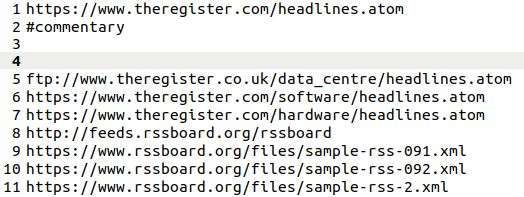
\includegraphics[width=0.8\linewidth]{img/feedfile.JPG}

    %%%%%%%%%%%%%%%%%%%%%%%%%%%%%%%%%%%%%%%
    %%%%%%%%%%%%%% Preklad %%%%%%%%%%%%%%
    \section{Preklad progrmau}
    \label{compile}
    Preklad programu je možný 2 spôsobmi:
    
    \subsection{Preklad cez príkazový riadok}
    \label{terminal}
    Pre preklad stačí na príkazový riadok napísať príkaz: \\
    
    \texttt{g++ -Wall -Wextra -Werror -pedantic -I /usr/include/libxml2/ -o feedreader ./src/feedreader.cpp -lcrypto -lssl -lxml2} \\
    
    Program je prekladaný ekvivalentom k prekladaču \texttt{gcc} - \texttt{g++}. Pri preklade sú použité všetky možnosti zachytávania chýb.
    
    \subsection{Použitie \texttt{Makefile}}
    \label{makefile}
    Pre preklad pomocou \texttt{Makefile} stačí na príkazový riadok napísať príkaz \texttt{make} alebo \texttt{make all}.

    %%%%%%%%%%%%%%%%%%%%%%%%%%%%%%%%%%%%%%%
    %%%%%%%%%%%%%%% Výstup %%%%%%%%%%%%%%%%
    \section{Výstup programu}
    \label{output}
    Na štandardný výstup sa vypíše názov zdroja uvedený \uv{***} a ukončený \uv{***}, napr. \textit{*** Príklad ***}. Na ďálších riadkoch budú uvedené názvy jedntolivých záznamov, ktoré budú oddelené prázdnym riadkom.
    V prípade zadania parametrov \texttt{-T}, \texttt{-a} alebo \texttt{-u}, budú pod názvom záznamu uvedené dodatočné informácie uvedené reťazcom \uv{Updated:}, \uv{Author:} resp. \uv{URL:}. Ak názov záznamu nebol uvedený vypíše sa reťazec \texttt{<No Title>}. Príklad výstupu: \\

    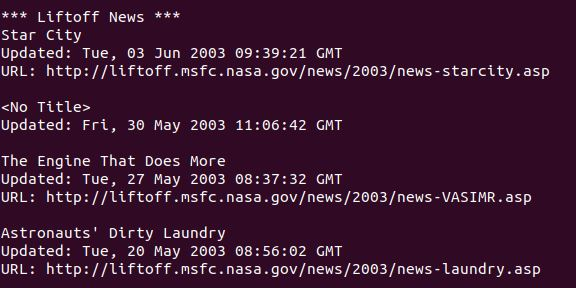
\includegraphics[width=0.8\linewidth]{img/output.JPG}

    %%%%%%%%%%%%%%%%%%%%%%%%%%%%%%%%%%%%%%%
    %%%%%%%%%%%%%% Testovanie %%%%%%%%%%%%%
    \section{Testovanie}
    Pre účely testovania som vytvoril skript \texttt{test.sh}, ktorý rekurzívne vyhľadá všetky súbory \texttt{feedfile} v zadanom adresári. Výsledky testov uloží do priečinka \texttt{test\_outputs} do súborov s príponami \texttt{.err} a \texttt{.out}. Tieto výstupné súbory sú nazvané podľa originálneho názvu \texttt{feedfile}, napr. ak má \texttt{feedfile} názov \texttt{abc.txt}, tak v súbore \texttt{test\_outputs} vzniknú 3 súbory:
    \begin{itemize}
        \item \texttt{abc\_c-Input.out} - v tomto súbore budú uložené výstupy všetkých záznamov, pri ktorých nenastala chyba
        \item \texttt{abc\_w-Input.out} - v tomto súbore budú uložené chybové hlásenia z rôznych nevalidných vstupov
        \item \texttt{abc\_c-Input.err} - v tomto súbore budú uložené chybové hlásenia záznamov, pri ktorých nastala chyba aj napriek validnému vstupu
    \end{itemize}
    
	Testovací skript je možné spustiť príkazom \texttt{make test} alebo \texttt{./test.sh [--nodir] [-d <addr>]}, kde \texttt{--nodir} zabezpečí vymazanie obsahu celého priečinka \texttt{test\_outputs} a \texttt{<addr>} je cesta k adresáru so súbormi \texttt{feedfile}. Ak nebude zadaný parameter \texttt{-d}, tak bude implicitne použitý aktuálny adresár. \\ 
	
    Pre vypísanie nápovedy testovacieho skriptu stačí použiť príkaz \texttt{make test\_help} alebo spustiť skript s parametrom \texttt{-h} alebo \texttt{--help}.    

	 %%%%%%%%%%%%%%%%%%%%%%%%%%%%%%%%%%%%%%%
    %%%%%%%%%%%%%%%% Záver %%%%%%%%%%%%%%%%
    \section{Záver}
    \label{endeSchluss}
    V projekte sa mi podarilo implementovať všetky časti aplikácie, ktoré boli v zadaní projektu. Testovanie nebolo veľmi rozsiahle, ale myslím že testy pokryli väčšinu validných i nevalidných vstupov. \\
    
     Samotný projekt nebol veľmi časovo náročný (približne 40 - 50 hodín), avšak mne osobne najviac času zabralo naštudovanie potrebných informácii napr. ako funguje knižnica \texttt{OpenSSL}, knižnica \texttt{libxml2} alebo formáty \texttt{Atom} a \texttt{RSS2.0}, čo mi zabralo ešte nejakých 5 - 10 hodín navyše. \\

    V každom prípade som si pri práci zdokonalil svoje vedomosti v oblasti zabezpečenej a nezabezpečenej internetovej komunikácii, ako funguje TLS a overovanie certifikátov alebo aké sú možnosti vytvárania \textit{feedov}. Ale hlavne som sa zdokonalil v programovaní v C++. Vyskúšal som prvýkrát OO prístup v C++ a využíval som množstvo regulárnych výrazov vďaka knižnici \texttt{<regex.h>}. Takisto som si rozšíril vedomosti o nové druhy súborov na štýl XML - \texttt{Atom} a \texttt{RSS2.0}. V neposlednom rade som sa naučil základy vytvárania dokumentu v programe \LaTeX, čo určite využijem pri vytváraní BP.

    %%%%%%%%%%%%%%%%%%%%%%%%%%%%%%%%%%%%%%%
    %%%%%%%%%%%%%% Zdroje %%%%%%%%%%%%%%%%%
    \clearpage
    \renewcommand{\refname}{Zdroje}
    \bibliographystyle{plain}
    \bibliography{reference}
 
\end{document}
